\chapter{Class Diagram and CRC card}

\section{Class Diagram}

\begin{figure}[h]
\begin{center}
  % Requires \usepackage{graphicx}
  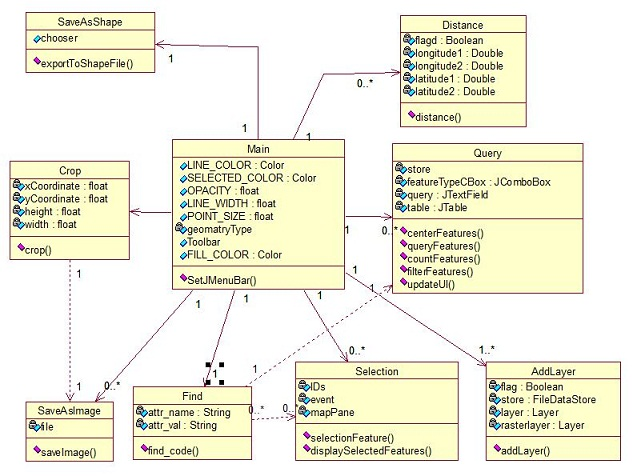
\includegraphics[scale=0.8] {Class.jpg}
  \caption [Class Diagram]{class diagram of entire system}
\end{center}
\end{figure}

\section{CRC Index Card}

\begin{table}[h]
\begin{tabular}{|p{7cm}|p{7cm}|}
  \hline
  % after \\: \hline or \cline{col1-col2} \cline{col3-col4} ...
  \multicolumn{2}{|l|}{ Class Name : Main} \\
  \hline
  \multicolumn{2}{|l|}{ Class Type : interaction, connection} \\
  \hline
  \multicolumn{2}{|l|}{ Class Characteristics : secure, sequential, permanent} \\
  \hline
  Responsibilities & Collaborators  \\
  \hline
  Create main window & Selection \\
  Open layers & Find \\
   & Save as Image\\
   & Crop \\
   & Add Layer \\
   & Query \\
   & Distance \\
  \hline
\end{tabular}
\caption[CRC card - Main Class]{CRC card - Main}
\end{table}

\begin{table}[h]
\begin{tabular}{|p{7cm}|p{7cm}|}
  \hline
  % after \\: \hline or \cline{col1-col2} \cline{col3-col4} ...
  \multicolumn{2}{|l|}{ Class Name :   Selection} \\
  \hline
  \multicolumn{2}{|l|}{ Class Type : interaction, connection} \\
  \hline
  \multicolumn{2}{|l|}{ Class Characteristics : secure, sequential, temporary} \\
  \hline
  Responsibilities & Collaborators  \\
  \hline
  Make selection of raster file & Find \\
  Make selection of vector file & \\
  \hline
\end{tabular}
\caption[CRC card - Selection]{CRC card - Selection}
\end{table}

\begin{table}[h]
\begin{tabular}{|p{7cm}|p{7cm}|}
  \hline
  % after \\: \hline or \cline{col1-col2} \cline{col3-col4} ...
  \multicolumn{2}{|l|}{ Class Name : Query} \\
  \hline
  \multicolumn{2}{|l|}{ Class Type : interaction, connection} \\
  \hline
  \multicolumn{2}{|l|}{ Class Characteristics : secure, sequential, temporary} \\
  \hline
  Responsibilities & Collaborators  \\
  \hline
  Get feature from Layer  & Main\\
  Apply query on feature & \\
  \hline
\end{tabular}
\caption[CRC card - Query]{CRC card - Query}
\end{table}

\begin{table}[h]
\begin{tabular}{|p{7cm}|p{7cm}|}
  \hline
  % after \\: \hline or \cline{col1-col2} \cline{col3-col4} ...
  \multicolumn{2}{|l|}{ Class Name : Save as Shape} \\
  \hline
  \multicolumn{2}{|l|}{ Class Type : interaction, device} \\
  \hline
  \multicolumn{2}{|l|}{ Class Characteristics : secure, sequential, permanent} \\
  \hline
  Responsibilities & Collaborators  \\
  \hline
  Get the name of layer & jMapFrame \\
  Get the name of selected feature & jLayerTable \\
  Get name of new layer & \\
  Read the content of selected attribute & \\
  Write the content into new layer & \\
  \hline
\end{tabular}
\caption[CRC card - Save as Shape]{CRC card - Save as Shape}
\end{table}

\begin{table}[h]
\begin{tabular}{|p{7cm}|p{7cm}|}
  \hline
  % after \\: \hline or \cline{col1-col2} \cline{col3-col4} ...
  \multicolumn{2}{|l|}{ Class Name : Save as Image} \\
  \hline
  \multicolumn{2}{|l|}{ Class Type : interaction, device} \\
  \hline
  \multicolumn{2}{|l|}{ Class Characteristics : secure, sequential, permanent} \\
  \hline
  Responsibilities & Collaborators  \\
  \hline
  Get the name of layer & \\
  Get the content of mapframe & \\
  Get name of new imagefile & \\
  Read the content of frame & \\
  Write the content into local file as image & \\
  \hline
\end{tabular}
\caption[CRC card - Save as Image]{CRC card - Save as Image}
\end{table}

\begin{table}[h]
\begin{tabular}{|p{7cm}|p{7cm}|}
  \hline
  % after \\: \hline or \cline{col1-col2} \cline{col3-col4} ...
  \multicolumn{2}{|l|}{ Class Name : Distance} \\
  \hline
  \multicolumn{2}{|l|}{ Class Type : interaction, connection} \\
  \hline
  \multicolumn{2}{|l|}{ Class Characteristics : secure, sequential, permanent} \\
  \hline
  Responsibilities & Collaborators  \\
  \hline
  Get the points & Main \\
  Apply the algorithm & \\
  Display result in Km. & \\
  \hline
\end{tabular}
\caption[CRC card - Distance]{CRC card - Distance}
\end{table}

\begin{table}[t]
\begin{tabular}{|p{7cm}|p{7cm}|}
  \hline
  % after \\: \hline or \cline{col1-col2} \cline{col3-col4} ...
  \multicolumn{2}{|l|}{ Class Name : Crop} \\
  \hline
  \multicolumn{2}{|l|}{ Class Type : interaction, connection, device} \\
  \hline
  \multicolumn{2}{|l|}{ Class Characteristics : secure, sequential, permanent} \\
  \hline
  Responsibilities & Collaborators  \\
  \hline
  Get the cropping parameter & Main \\
  Save the temporary result in image & save as image \\
  Crop that image & \\
  Save the Cropped result in Local file & \\
  \hline
\end{tabular}
\caption[CRC card - Crop]{CRC card - Crop}
\end{table}
